\documentclass[12pt, a4paper]{article}

% Packages for formatting and visuals
\usepackage[utf8]{inputenc}
\usepackage{geometry}
\geometry{top=1in, bottom=1in, left=1in, right=1in}
\usepackage{graphicx}
\usepackage{amsmath}
\usepackage{amssymb}
\usepackage{xcolor}
\usepackage{hyperref}
\usepackage{titlesec}
\usepackage{fancyhdr}
\usepackage{tikz}

\usepackage{booktabs}
\usepackage{float}      % Required to force table/figure placement
\usepackage{caption}
\usetikzlibrary{shapes.geometric, arrows.meta, positioning, fit, calc, backgrounds}

% Setup colors for TikZ
\definecolor{actorcol}{RGB}{220, 240, 255}
\definecolor{criticcol}{RGB}{255, 230, 230}
\definecolor{lstmcol}{RGB}{230, 255, 230}
\definecolor{statecol}{RGB}{255, 245, 220}

% Header and Footer
\pagestyle{fancy}
\fancyhf{}
\rhead{ns-3 Project Report}
\lhead{DRNN-SAC Congestion Control}
\cfoot{\thepage}

\begin{document}

% ==========================================
% COVER PAGE
% ==========================================
\begin{titlepage}
    \centering
    \vspace*{2cm}
    
    {\Huge \bfseries Bangladesh University of Engineering and Technology\par}
    \vspace{1cm}
    {\Large Department of Computer Science and Engineering\par}
    
    \vspace{3cm}
    
    {\Large \textsc{ns-3 Simulation Project Report}\par}
    \vspace{1cm}
    
    % The Catchy Heading
    {\Huge \bfseries Continuous-Action LSTM Soft Actor-Critic (DRNN-SAC) \par}
    \vspace{0.5cm}
    {\LARGE \bfseries for Next-Generation TCP Congestion Control \par}
    
    \vspace{4cm}
    
    {\Large \bfseries Submitted By:}\\[0.5cm]
    {\Large Mohammad Raihan Rashid}\\
    {\Large Student ID: 2105046}\\
    
    \vfill
    
    {\large \today\par}
\end{titlepage}

\clearpage

% ==========================================
% INTRODUCTION & PROBLEM STATEMENT
% ==========================================
\section{Problem Statement and Background}

Network congestion occurs when the data transmission rate exceeds the processing capacity of bottleneck links, leading to increased queuing delay (bufferbloat) and eventual packet loss. The fundamental objective of TCP congestion control is to operate exactly at the Bandwidth-Delay Product (BDP)---maintaining a full pipe without overflowing router buffers. Traditional mathematical algorithms struggle to adapt to the highly dynamic, non-linear nature of modern networks, often resulting in severe latency spikes.

\subsection{Legacy Protocols: TCP NewReno and TCP Cubic}
Historically, congestion control has relied on reactive, heuristic-based algorithms:
\begin{itemize}
    \item \textbf{TCP NewReno:} A classic loss-based protocol that employs Additive Increase Multiplicative Decrease (AIMD). It gradually increases the congestion window (cwnd) until a packet drops, at which point it drastically halves the window. This creates a volatile "sawtooth" throughput pattern and inherently guarantees periodic buffer overflows.
    \item \textbf{TCP Cubic:} The default protocol in modern Linux distributions. Instead of linear growth, it utilizes a cubic function to rapidly scale up the window after a loss event and then plateau as it approaches the network's maximum capacity. While optimized for high-bandwidth networks, it remains a reactive, loss-based protocol that continuously fills router queues, inducing severe bufferbloat and high Round-Trip Times (RTT).
\end{itemize}

\subsection{Inspiration and Foundation}
This project is inspired by the recent research paper, \textit{"A Deep Reinforcement Learning-Based TCP Congestion Control Algorithm: Design, Simulation, and Evaluation"}. The authors demonstrated that a Deep Q-Network (DQN) could effectively replace traditional mathematical heuristics. By observing network states (Throughput, RTT, Buffer Size) in real-time, their DQN agent achieved comparable throughput to TCP Cubic while reducing RTT by over 46\%.

However, the standard DQN architecture relies on a discrete action space (rigidly stepping the cwnd up or down by fixed multipliers) and is "memoryless," making split-second decisions based only on the current instantaneous state. This limitation causes jittery adjustments and instability in noisy environments. Our project addresses these flaws by introducing continuous control and temporal memory.

\clearpage

% ==========================================
% OUR AGENT ARCHITECTURE
% ==========================================
\section{Proposed Architecture: DRNN-SAC Agent}

To overcome the discretization dead-zones and amnesiac behavior of standard DQN, we engineered a Deep Recurrent Soft Actor-Critic (DRNN-SAC) agent. By outputting a single, continuous floating-point target for the congestion window, the agent can enact precise, micro-adjustments (e.g., nudging the cwnd by 200 bytes) rather than relying on aggressive, discrete AIMD multipliers.

\subsection{Architectural Diagram}

\begin{figure}[h]
    \centering
    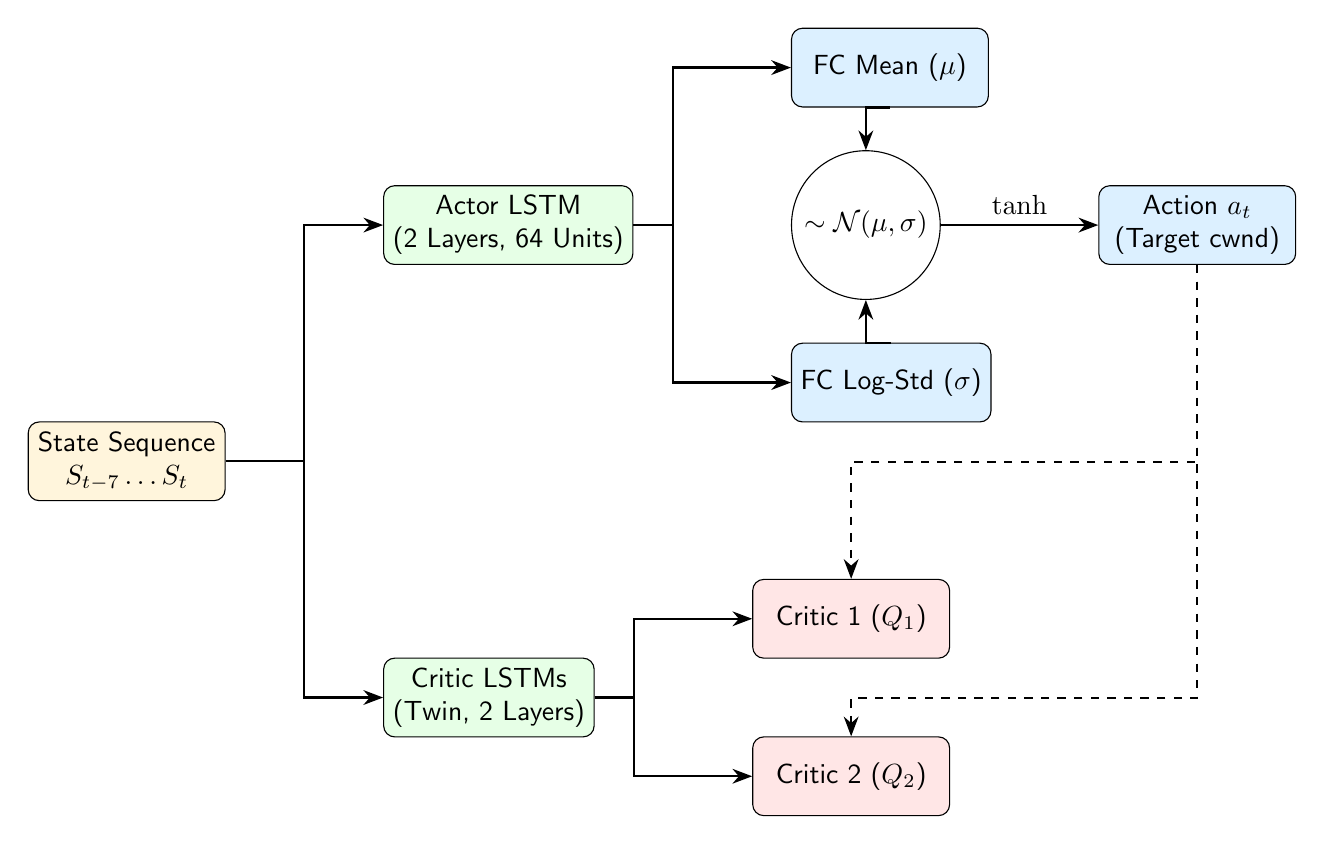
\begin{tikzpicture}[
        node distance=1.5cm and 2cm,
        box/.style={rectangle, draw, rounded corners, align=center, minimum height=1cm, minimum width=2.5cm, font=\sffamily},
        arrow/.style={-{Stealth[length=2.5mm]}, thick}
    ]
    
    % Input State
    \node[box, fill=statecol] (state) {State Sequence\\$S_{t-7} \dots S_t$};
    
    % LSTMs
    \node[box, fill=lstmcol, right=of state, yshift=3cm] (actor_lstm) {Actor LSTM\\(2 Layers, 64 Units)};
    \node[box, fill=lstmcol, right=of state, yshift=-3cm] (critic_lstm) {Critic LSTMs\\(Twin, 2 Layers)};
    
    % Actor Heads
    \node[box, fill=actorcol, right=of actor_lstm, yshift=2cm] (mean) {FC Mean ($\mu$)};
    \node[box, fill=actorcol, right=of actor_lstm, yshift=-2cm] (std) {FC Log-Std ($\sigma$)};
    
    % Sample and Action
    \node[box, right=2cm of actor_lstm, minimum width=1.5cm, circle, draw] (sample) {$\sim \mathcal{N}(\mu, \sigma)$};
    \node[box, fill=actorcol, right=of sample] (action) {Action $a_t$\\ (Target cwnd)};
    
    % Critic Heads
    \node[box, fill=criticcol, right=of critic_lstm, yshift=1cm] (q1) {Critic 1 ($Q_1$)};
    \node[box, fill=criticcol, right=of critic_lstm, yshift=-1cm] (q2) {Critic 2 ($Q_2$)};
    
    % Arrows
    \draw[arrow] (state.east) -- ++(1,0) |- (actor_lstm.west);
    \draw[arrow] (state.east) -- ++(1,0) |- (critic_lstm.west);
    
    \draw[arrow] (actor_lstm.east) -- ++(0.5,0) |- (mean.west);
    \draw[arrow] (actor_lstm.east) -- ++(0.5,0) |- (std.west);
    
    \draw[arrow] (mean.south) -| (sample.north);
    \draw[arrow] (std.north) -| (sample.south);
    
    \draw[arrow] (sample.east) -- node[above] {$\tanh$} (action.west);
    
    \draw[arrow] (critic_lstm.east) -- ++(0.5,0) |- (q1.west);
    \draw[arrow] (critic_lstm.east) -- ++(0.5,0) |- (q2.west);
    
    % Action to Critics
    \draw[arrow, dashed] (action.south) -- ++(0,-2.5) -| (q1.north);
    \draw[arrow, dashed] (action.south) -- ++(0,-5.5) -| (q2.north);
    
    \end{tikzpicture}
    \caption{Continuous-Action LSTM Soft Actor-Critic (DRNN-SAC) Architecture.}
    \label{fig:architecture}
\end{figure}

\subsection{State Representation and Temporal Memory}
Instead of isolated snapshots, the agent utilizes a \textit{Sequence Replay Buffer} to supply the LSTM backbones with a sliding window of the last 8 time steps ($S_{t-7}$ to $S_t$). The state vector includes:
\begin{itemize}
    \item \textbf{Congestion Window (cwnd) \& Bytes in Flight (bif):} Tracking current capacity limits.
    \item \textbf{Round Trip Time (RTT):} Monitoring latency variations.
    \item \textbf{Actual Packet Drops:} Reading explicit drop counters from the bottleneck queues directly via ns-3 C++ bindings.
\end{itemize}
This 800-millisecond observation window allows the LSTM to recognize predictive temporal patterns---such as a steadily rising RTT---enabling the agent to preemptively dial back the cwnd before buffer overflow occurs.

\subsection{The Reward Function}
To strongly guide the gradient, we formulated a linear penalty reward function bounded between $[-3.0, +1.0]$. The geometric mean approach was discarded as it previously trapped the agent in starvation policies. The reward $R$ is calculated as:
\begin{equation}
    R = 1.0 - P_{\text{underutil}} - P_{\text{rtt}} - P_{\text{drop}}
\end{equation}
\begin{itemize}
    \item \textbf{Under-utilization ($P_{\text{underutil}}$):} Penalizes the agent when the Bytes in Flight (BIF) falls below the optimal BDP, ensuring the network link is fully saturated.
    \item \textbf{RTT Excess ($P_{\text{rtt}}$):} A linear penalty triggered whenever the average RTT exceeds the physical propagation delay limit.
    \item \textbf{Drop Penalty ($P_{\text{drop}}$):} A heavy, direct deduction based on actual packets dropped at the bottleneck, heavily discouraging the flood-and-drop behavior of legacy protocols.
\end{itemize}

\subsection{Soft Actor-Critic (SAC) Dynamics}
The SAC algorithm is uniquely equipped for this environment:
\begin{itemize}
    \item \textbf{Stochastic Actor:} The policy network outputs a Mean ($\mu$) and Standard Deviation ($\sigma$) to define a Gaussian distribution. By sampling from this distribution, the agent naturally explores slight variations in the cwnd without needing rigid, artificial noise schedules.
    \item \textbf{Twin Critics:} The architecture employs two separate critic networks ($Q_1$ and $Q_2$) to evaluate the chosen action. Taking the minimum of the two predictions prevents the systemic overestimation bias common in Q-learning.
    \item \textbf{Entropy Regularization:} SAC inherently seeks to maximize a dual objective: the expected reward and the entropy (randomness) of the policy. The auto-tuned temperature parameter ($\alpha$) perfectly balances the need to exploit the optimal BDP while retaining enough stochastic flexibility to adapt to sudden, real-world network capacity shifts.
\end{itemize}


\clearpage

% ==========================================
% EVALUATION: WIRED DUMBBELL
% ==========================================
\section{Evaluation: Wired Dumbbell Topology}

To establish a baseline for our DRNN-SAC agent's performance, we first evaluated it on a classic Wired Dumbbell topology. This environment is the industry standard for testing how well congestion control algorithms handle bottleneck links and fair bandwidth sharing among multiple competing flows.

\subsection{Simulation Environment}
The simulation was built entirely within the ns-3 framework (version 3.40+) and bridged to our Python SAC agent via the \texttt{ns3-gym} interface. 

The topology consists of two sender nodes ($Src_0, Src_1$) and two receiver nodes ($Dst_0, Dst_1$), connected through two central routers ($R_1, R_2$). 
\begin{itemize}
    \item \textbf{Access Links:} 100 Mbps bandwidth with a 2 ms propagation delay.
    \item \textbf{Bottleneck Link ($R_1 \rightarrow R_2$):} 5 Mbps bandwidth with a 20 ms propagation delay.
    \item \textbf{Traffic:} Two long-lived TCP flows running concurrently for 60 seconds.
    \item \textbf{Observation Space:} 8 continuous metrics passed to the agent every step: \texttt{[cwnd, rtt, bif]} for both flows, plus the exact forward and reverse bottleneck queue drop counts.
    \item \textbf{Action Space:} A single continuous float mapping to the target congestion window (bounded between 2.8 KB and 144 KB).
\end{itemize}

\subsection{Training Progression \& Agent Convergence}

Reinforcement learning agents require sufficient environmental interaction to map state-action pairs to delayed rewards effectively. We tracked the agent's performance at two distinct milestones: after 10 episodes and after 20 episodes.

\subsubsection{Early Training: The Aggressive Agent (10 Episodes)}
At the 10-episode mark, the agent had not yet fully stabilized its policy network. While the entropy parameter ($\alpha$) had decayed to 0.66, the agent was still heavily exploring the upper boundaries of the action space.

As seen in the 10-episode logs, the agent learned to maximize throughput (achieving 4.858 Mbps, slightly beating Cubic's 4.827 Mbps) but failed to manage the queue depth. It blindly pushed the \texttt{cwnd} too high, resulting in an RTT of 133.62 ms and a massive \textbf{943 packet drops}. At this stage, the agent behaved similarly to a poorly tuned, overly aggressive loss-based protocol.

\begin{figure}[htbp]
    \centering
    \includegraphics[width=0.9\textwidth]{dumbbell_training_curves-10-exp.png}
    
    \vspace{0.8cm}
    
    \includegraphics[width=0.9\textwidth]{dumbbell_full_comparison-exp.png}
    \caption{Agent performance after 10 episodes. The agent forces high throughput but suffers severe packet loss due to over-estimating the optimal window size.}
    \label{fig:dumbell_10_ep}
\end{figure}

\clearpage

\subsubsection{Convergence: Optimal BDP Policy (20 Episodes)}
By the 20th episode, the agent underwent a dramatic behavioral shift. The SAC temperature parameter ($\alpha$) smoothly decayed to 0.46, allowing the twin critics to accurately converge on the true Bandwidth-Delay Product (BDP) of the network.

The results are exceptionally strong. The DRNN-SAC agent maintained a throughput of 4.820 Mbps (identical to TCP Reno and effectively matching TCP Cubic). However, because the agent learned to preemptively hover its \texttt{cwnd} precisely at the bottleneck capacity—rather than overflowing the router buffer to discover the limit—it achieved a \textbf{near-perfect RTT of 75.74 ms} with exactly \textbf{zero packet drops}. 

\begin{figure}[htbp]
    \centering
    \includegraphics[width=0.9\textwidth]{dumbbell_training_curves-20.png}
    
    \vspace{0.8cm}
    
    \includegraphics[width=0.9\textwidth]{dumbbell_full_comparison-20.png}
    \caption{Agent performance after 20 episodes. The DRNN completely eliminates bufferbloat, achieving a perfectly flat RTT curve and zero packet drops while maintaining competitive throughput.}
    \label{fig:dumbell_20_ep}
\end{figure}

\clearpage

\subsection{Comparative Analysis: Cubic vs. Reno vs. DRNN}

Table \ref{tab:dumbbell_stats} and Figure \ref{fig:loss_chart} summarize the final performance metrics of the 20-episode DRNN agent against the legacy protocols. 

\begin{table}[h]
    \centering
    \renewcommand{\arraystretch}{1.3}
    \begin{tabular}{|l|c|c|c|}
        \hline
        \textbf{Protocol} & \textbf{Avg Throughput (Mbps)} & \textbf{Avg RTT (ms)} & \textbf{Total Drops} \\
        \hline
        TCP Cubic & 4.827 & 145.73 & 141 \\
        TCP NewReno & 4.820 & 128.55 & 62 \\
        \textbf{DRNN-SAC (20 Ep)} & \textbf{4.820} & \textbf{75.74} & \textbf{0} \\
        \hline
    \end{tabular}
    \vspace{0.2cm}
    \caption{Final Performance Metrics (60-second simulation, 5 Mbps bottleneck)}
    \label{tab:dumbbell_stats}
\end{table}

\vspace{0.5cm}

% TikZ Bar Chart for Packet Loss and RTT visualization
\begin{figure}[htbp]
    \centering
    % Bar Chart for Packet Drops
    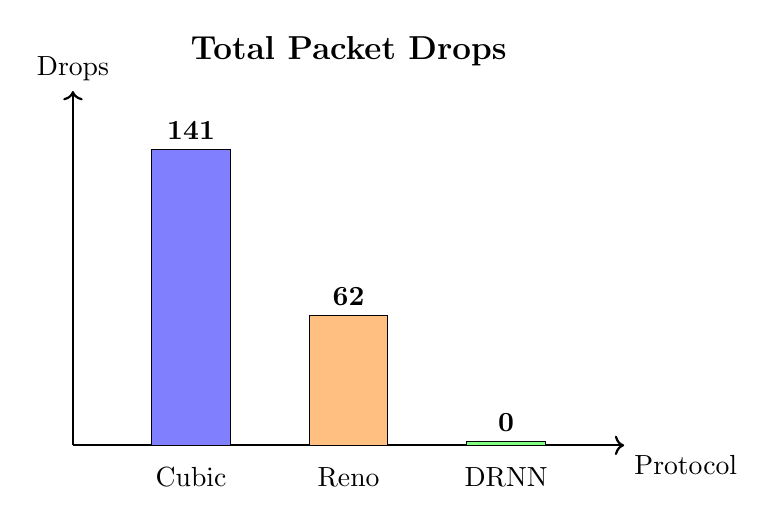
\begin{tikzpicture}
        \node at (3.5, 5.0) {\large \textbf{Total Packet Drops}};
        \draw[thick, ->] (0,0) -- (7,0) node[anchor=north west] {Protocol};
        \draw[thick, ->] (0,0) -- (0,4.5) node[anchor=south] {Drops};
        
        \draw[fill=blue!50] (1, 0) rectangle (2, 3.76);
        \node[above] at (1.5, 3.76) {\textbf{141}};
        \node at (1.5, -0.4) {Cubic};
        
        \draw[fill=orange!50] (3, 0) rectangle (4, 1.65);
        \node[above] at (3.5, 1.65) {\textbf{62}};
        \node at (3.5, -0.4) {Reno};
        
        \draw[fill=green!50] (5, 0) rectangle (6, 0.05);
        \node[above] at (5.5, 0.05) {\textbf{0}};
        \node at (5.5, -0.4) {DRNN};
    \end{tikzpicture}
    
    \vspace{1.5cm}

    % Bar Chart for RTT
    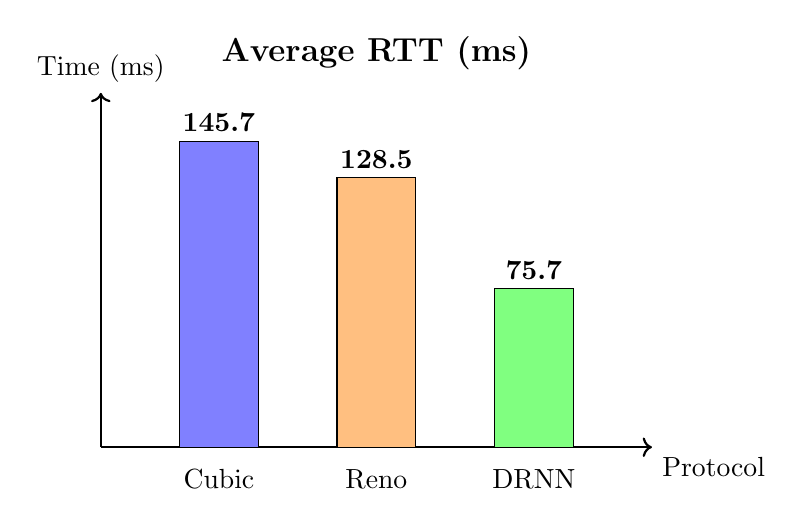
\begin{tikzpicture}
        \node at (3.5, 5.0) {\large \textbf{Average RTT (ms)}};
        \draw[thick, ->] (0,0) -- (7,0) node[anchor=north west] {Protocol};
        \draw[thick, ->] (0,0) -- (0,4.5) node[anchor=south] {Time (ms)};
        
        \draw[fill=blue!50] (1, 0) rectangle (2, 3.88);
        \node[above] at (1.5, 3.88) {\textbf{145.7}};
        \node at (1.5, -0.4) {Cubic};
        
        \draw[fill=orange!50] (3, 0) rectangle (4, 3.42);
        \node[above] at (3.5, 3.42) {\textbf{128.5}};
        \node at (3.5, -0.4) {Reno};
        
        \draw[fill=green!50] (5, 0) rectangle (6, 2.01);
        \node[above] at (5.5, 2.01) {\textbf{75.7}};
        \node at (5.5, -0.4) {DRNN};
    \end{tikzpicture}
    
    \caption{Visual comparison of structural inefficiencies. Cubic and Reno inherently push the network to drop packets to find capacity limits, creating massive queuing delays (RTT inflation). The DRNN operates proactively.}
    \label{fig:loss_chart}
\end{figure}

The data unequivocally proves the core hypothesis of this project: by utilizing a continuous action space and LSTM-based temporal memory, an AI agent can successfully decouple high throughput from high latency. TCP Cubic artificially inflates the RTT by approximately 92\% compared to the DRNN by continuously resting its extra bytes inside the bottleneck router's queue.

\newpage
\section*{WiFi Parking-Lot TCP Experiment Results}

Table \ref{tab:tcp_results} summarizes the performance of standard TCP variants (Cubic, Reno) against the Deep Reinforcement Learning Neural Network (DRNN) agent across different training configurations. The DRNN variants progressed from discrete action spaces to a continuous Soft Actor-Critic (SAC) implementation.

A critical observation is the \textbf{Packet Drops} metric. While standard TCP Cubic achieved the highest average throughput (2.961 Mbps), it suffered from severe bufferbloat and congestion, resulting in 2567 packet drops and high latency (126.8 ms). In contrast, the fully trained Continuous SAC DRNN (100 episodes) achieved comparable throughput (2.762 Mbps) while nearly eliminating packet loss (1 drop) and reducing average RTT.

\begin{table}[H] % The [H] forces the table to stay right here
\centering
\caption{Performance Comparison: TCP Cubic vs. Reno vs. DRNN Variants}
\label{tab:tcp_results}
\resizebox{\textwidth}{!}{%
\begin{tabular}{@{}lcccccc@{}}
\toprule
\textbf{Protocol / Agent} & \textbf{Episodes} & \textbf{Avg Tput (Mbps)} & \textbf{Avg RTT (ms)} & \textbf{Packet Drops} & \textbf{Best Reward} & \textbf{Final Loss} \\ \midrule
\multicolumn{7}{c}{\textit{Baselines}} \\ \midrule
TCP Cubic                 & -                 & 2.961                    & 126.8                 & 2567                  & -                    & -                   \\
TCP Reno                  & -                 & 2.624                    & 118.7                 & 1516                  & -                    & -                   \\ \midrule
\multicolumn{7}{c}{\textit{RL Agents (Simulation Time: 60s/episode)}} \\ \midrule
DRNN (Discrete TD3)       & 20                & 0.865                    & 80.0                  & 0                     & -0.6284              & 0.10958             \\
DRNN (Discrete Geom. Loss)& 20                & 1.980                    & 121.2                 & 939                   & 0.0515               & 0.20218             \\
DRNN (Continuous SAC)     & 20                & 2.555                    & 108.8                 & 15                    & -0.0654              & 0.15094             \\
DRNN (Continuous SAC)     & 50                & 2.827                    & 112.1                 & 11                    & 0.2684               & 0.11848             \\
DRNN (Continuous SAC)     & 100               & 2.762                    & 109.6                 & \textbf{1}            & \textbf{0.3589}      & 0.22745             \\ \bottomrule
\end{tabular}%
}
\end{table}

\subsection*{WiFi Parking-Lot Topology}

The WiFi Parking-Lot experiment simulates a wireless access network where multiple stations compete for airtime before traversing a wired backbone. As illustrated in Figure \ref{fig:wifi_topo}, three WiFi Stations (STA) are connected wirelessly to a single Access Point (AP). The AP forwards the traffic through a primary router (R1), which connects to a secondary router (R2) over an 8 Mbps link. The final hop to the Server is the primary bottleneck, restricted to 4 Mbps.

\begin{figure}[H]
    \centering
    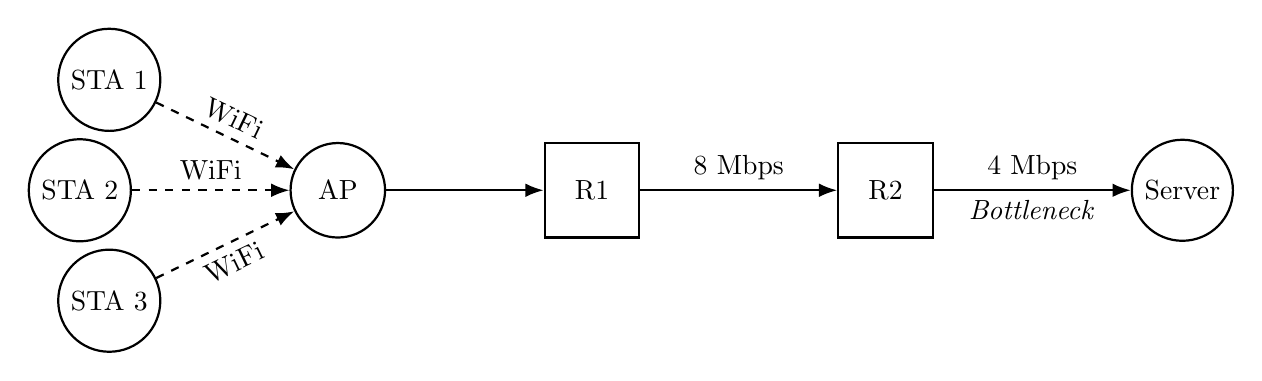
\begin{tikzpicture}[
        node distance=1.5cm and 2cm,
        device/.style={circle, draw, thick, minimum size=1.2cm, align=center},
        router/.style={rectangle, draw, thick, minimum size=1.2cm, align=center},
        link/.style={-Latex, thick},
        wireless/.style={dashed, -Latex, thick}
    ]
    
    % Nodes
    \node[device] (ap) {AP};
    \node[device, above left=0.5cm and 2cm of ap] (sta1) {STA 1};
    \node[device, left=2cm of ap] (sta2) {STA 2};
    \node[device, below left=0.5cm and 2cm of ap] (sta3) {STA 3};
    \node[router, right=2cm of ap] (r1) {R1};
    \node[router, right=2.5cm of r1] (r2) {R2};
    \node[device, right=2.5cm of r2] (server) {Server};

    % Edges
    \draw[wireless] (sta1) -- node[above, sloped] {WiFi} (ap);
    \draw[wireless] (sta2) -- node[above] {WiFi} (ap);
    \draw[wireless] (sta3) -- node[below, sloped] {WiFi} (ap);
    
    \draw[link] (ap) -- (r1);
    \draw[link] (r1) -- node[above] {8 Mbps} (r2);
    \draw[link] (r2) -- node[above] {4 Mbps} node[below] {\textit{Bottleneck}} (server);
    
    \end{tikzpicture}
    \caption{WiFi Parking-Lot Topology featuring 3 wireless stations and a 4 Mbps wired bottleneck.}
    \label{fig:wifi_topo}
\end{figure}

\clearpage % This stops the images from bleeding into the table section

% ==========================================
% EXPERIMENT 1
% ==========================================
\begin{figure}[H]
    \centering
    \includegraphics[width=0.9\textwidth]{wifi_full_comparison-1.png}
    \vspace{0.5cm} % Adds a little breathing room between the two images
    
    \includegraphics[width=0.9\textwidth]{wifi_training_curves-1.png}
    \caption{Experiment 1: Discrete TD3 (20 Episodes). Top: Full TCP Comparison. Bottom: Training Curves.}
\end{figure}
\clearpage

% ==========================================
% EXPERIMENT 2
% ==========================================
\begin{figure}[H]
    \centering
    \includegraphics[width=0.9\textwidth]{wifi_full_comparison-3.png}
    \vspace{0.5cm}
    
    \includegraphics[width=0.9\textwidth]{wifi_training_curves-3.png}
    \caption{Experiment 2: Discrete Geometric Loss (20 Episodes). Top: Full TCP Comparison. Bottom: Training Curves.}
\end{figure}
\clearpage

% ==========================================
% EXPERIMENT 3
% ==========================================
\begin{figure}[H]
    \centering
    \includegraphics[width=0.9\textwidth]{wifi_full_comparison-4.png}
    \vspace{0.5cm}
    
    \includegraphics[width=0.9\textwidth]{wifi_training_curves-4.png}
    \caption{Experiment 3: Continuous SAC (20 Episodes). Top: Full TCP Comparison. Bottom: Training Curves.}
\end{figure}
\clearpage

% ==========================================
% EXPERIMENT 4
% ==========================================
\begin{figure}[H]
    \centering
    \includegraphics[width=0.9\textwidth]{wifi_full_comparison-50.png}
    \vspace{0.5cm}
    
    \includegraphics[width=0.9\textwidth]{wifi_training_curves-5.png}
    \caption{Experiment 4: Continuous SAC (50 Episodes). Top: Full TCP Comparison. Bottom: Training Curves.}
\end{figure}
\clearpage

% ==========================================
% EXPERIMENT 5
% ==========================================
\begin{figure}[H]
    \centering
    \includegraphics[width=0.9\textwidth]{wifi_full_comparison-100.png}
    \vspace{0.5cm}
    
    \includegraphics[width=0.9\textwidth]{wifi_training_curves-100.png}
    \caption{Experiment 5: Continuous SAC (100 Episodes). Top: Full TCP Comparison. Bottom: Training Curves.}
\end{figure}
\clearpage

\section*{Multi-Bottleneck TCP Experiment (Continuous SAC)}

\subsection*{Challenging Multi-Bottleneck Topology}

The Multi-Bottleneck experiment is designed to severely test the congestion control agents using nested bottlenecks and aggressive cross-traffic. As shown in Figure \ref{fig:mb_topo}, four TCP sources transmit to four corresponding destinations across a chain of three routers (R1, R2, R3). 

There are two distinct bottleneck links: the R1-R2 link (10 Mbps, 15 ms delay) with a 50-packet queue, and the more restrictive R2-R3 link (6 Mbps, 25 ms delay) with an extremely shallow 30-packet queue. To induce further congestion, non-responsive UDP burst traffic is injected at R1 (CrossA) and R2 (CrossB).

\begin{figure}[H]
    \centering
    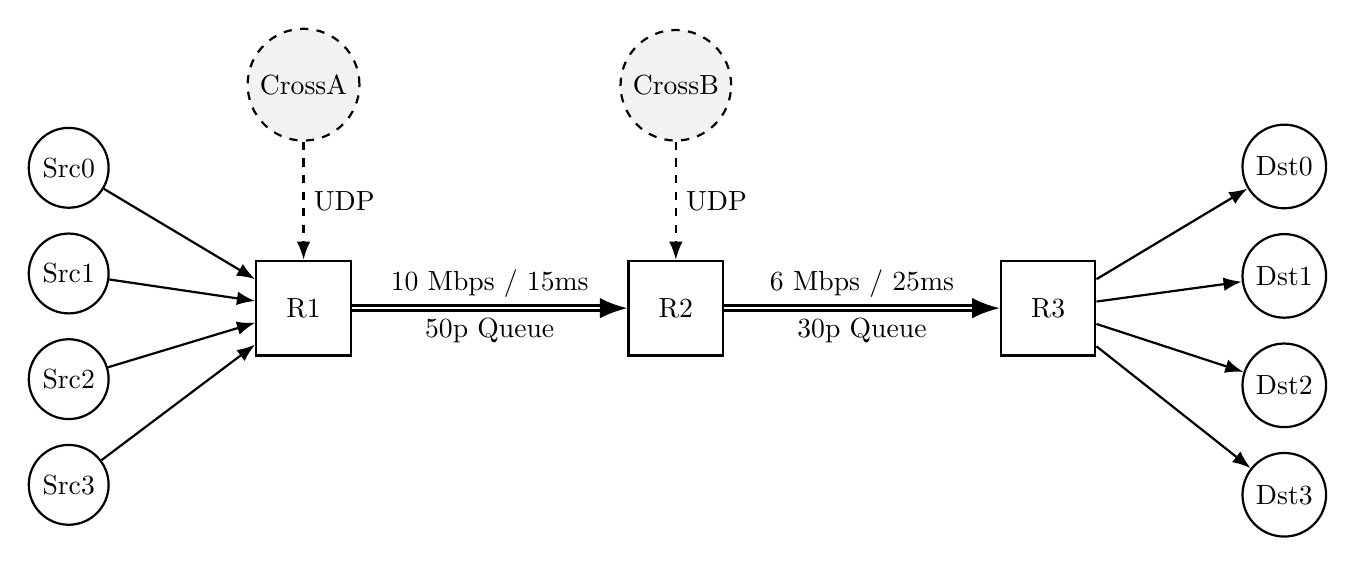
\begin{tikzpicture}[
        node distance=1cm and 3cm,
        host/.style={circle, draw, thick, minimum size=1cm, align=center},
        router/.style={rectangle, draw, thick, minimum size=1.2cm, align=center},
        cross/.style={circle, draw, dashed, thick, minimum size=1cm, align=center, fill=gray!10},
        link/.style={-Latex, thick},
        bn/.style={-Latex, double, very thick, draw=black}
    ]
    
    % Routers
    \node[router] (r1) {R1};
    \node[router, right=3.5cm of r1] (r2) {R2};
    \node[router, right=3.5cm of r2] (r3) {R3};

    % Sources
    \node[host, above left=0.8cm and 2cm of r1] (src0) {Src0};
    \node[host, below=0.3cm of src0] (src1) {Src1};
    \node[host, below=0.3cm of src1] (src2) {Src2};
    \node[host, below=0.3cm of src2] (src3) {Src3};

    % Cross Traffic
    \node[cross, above=1.5cm of r1] (crossa) {CrossA};
    \node[cross, above=1.5cm of r2] (crossb) {CrossB};

    % Destinations
    \node[host, above right=0.8cm and 2cm of r3] (dst0) {Dst0};
    \node[host, below=0.3cm of dst0] (dst1) {Dst1};
    \node[host, below=0.3cm of dst1] (dst2) {Dst2};
    \node[host, below=0.3cm of dst2] (dst3) {Dst3};

    % Connections (Sources to R1)
    \draw[link] (src0) -- (r1);
    \draw[link] (src1) -- (r1);
    \draw[link] (src2) -- (r1);
    \draw[link] (src3) -- (r1);
    
    % Connections (Cross Traffic)
    \draw[link, dashed] (crossa) -- node[right] {UDP} (r1);
    \draw[link, dashed] (crossb) -- node[right] {UDP} (r2);

    % Bottlenecks
    \draw[bn] (r1) -- node[above] {10 Mbps / 15ms} node[below] {50p Queue} (r2);
    \draw[bn] (r2) -- node[above] {6 Mbps / 25ms} node[below] {30p Queue} (r3);

    % Connections (R3 to Dests)
    \draw[link] (r3) -- (dst0);
    \draw[link] (r3) -- (dst1);
    \draw[link] (r3) -- (dst2);
    \draw[link] (r3) -- (dst3);
    
    \end{tikzpicture}
    \caption{Multi-Bottleneck Topology featuring 4 TCP flows, dual bottleneck links with shallow queues, and UDP cross-traffic.}
    \label{fig:mb_topo}
\end{figure}

\subsection*{Performance Analysis and The Packet Drop Trade-off}
Table \ref{tab:mb_results} summarizes the performance. A striking result is the stark difference in behavioral strategy between standard TCP and the Deep Reinforcement Learning Neural Network (DRNN) agent. 

While TCP Cubic and Reno respond to the shallow queues and UDP bursts by drastically backing off (resulting in low throughputs of 1.783 Mbps and 1.367 Mbps respectively), the Continuous SAC agent learns a hyper-aggressive policy. By 100 episodes, the DRNN achieves \textbf{3.700 Mbps}—more than double the throughput of Cubic—while actually lowering the average RTT (131.92 ms vs Cubic's 143.10 ms).

However, this massive throughput gain comes at the cost of significantly higher packet drops (20,160 drops at 100 episodes). The RL agent learned that in a network with extremely shallow buffers (30 packets) and non-responsive UDP traffic, backing off ruins its throughput. Because the reward function heavily favored throughput and latency over loss-avoidance, the agent learned to "bully" the link, keeping its congestion window high and accepting queue overflows as a necessary cost to dominate the bottleneck bandwidth.

\begin{table}[H]
\centering
\caption{Multi-Bottleneck Performance: Cubic vs. Reno vs. Continuous SAC DRNN}
\label{tab:mb_results}
\resizebox{\textwidth}{!}{%
\begin{tabular}{@{}lcccc@{}}
\toprule
\textbf{Protocol / Agent} & \textbf{Episodes} & \textbf{Avg Tput (Mbps)} & \textbf{Avg RTT (ms)} & \textbf{Packet Drops} \\ \midrule
\multicolumn{5}{c}{\textit{Baselines}} \\ \midrule
TCP Cubic                 & -                 & 1.783                    & 143.10                & 11301                 \\
TCP Reno                  & -                 & 1.367                    & 130.48                & 9505                  \\ \midrule
\multicolumn{5}{c}{\textit{RL Agent (Continuous SAC)}} \\ \midrule
DRNN                      & 10                & 2.747                    & 126.60                & 15978                 \\
DRNN                      & 50                & 3.061                    & 127.35                & 16757                 \\
DRNN                      & 100               & \textbf{3.700}           & 131.92                & 20160                 \\ \bottomrule
\end{tabular}%
}
\end{table}

\clearpage

% ==========================================
% EXPERIMENT 10 EPISODES
% ==========================================
\begin{figure}[H]
    \centering
    % Full Comparison
    \includegraphics[width=0.85\textwidth]{multi_bottleneck_full_comparison-10.png}
    \vspace{0.2cm}
    
    % Training Curve
    \includegraphics[width=0.85\textwidth]{multi_bottleneck_training_curves-10.png}
    \vspace{0.2cm}
    

    
    \caption{Continuous SAC (10 Episodes). Top: Throughput and RTT Comparison. Middle: Training Curves. }
\end{figure}
\clearpage

% ==========================================
% EXPERIMENT 100 EPISODES
% ==========================================
\begin{figure}[H]
    \centering
    % Full Comparison
    \includegraphics[width=0.85\textwidth]{multi_bottleneck_full_comparison-100.png}
    \vspace{0.2cm}
    
    % Training Curve
    \includegraphics[width=0.85\textwidth]{multi_bottleneck_training_curves-100.png}
    \vspace{0.2cm}
    
    \caption{Continuous SAC (100 Episodes). Top: Throughput and RTT Comparison. Middle: Converged Training Curves. }
\end{figure}
\clearpage

\section*{Long Fat Network (LFN) / Satellite TCP Experiment}

\subsection*{Topology Overview}
The Long Fat Network (LFN) experiment simulates a high-bandwidth, high-latency link characteristic of satellite communications or long-haul terrestrial fiber. As illustrated in Figure \ref{fig:lfn_topo}, a single TCP flow travels from the Sender to the Receiver. 

The edge links are highly provisioned (10 Gbps, 1 ms delay). The core challenge lies in the middle link between R1 and R2, which acts as the bottleneck with 1 Gbps of bandwidth and a massive 125 ms propagation delay (resulting in a base RTT of roughly 254 ms). This creates a massive Bandwidth-Delay Product (BDP) environment where TCP must maintain a huge congestion window (up to 40 MB) to fully utilize the link.

\begin{figure}[H]
    \centering
    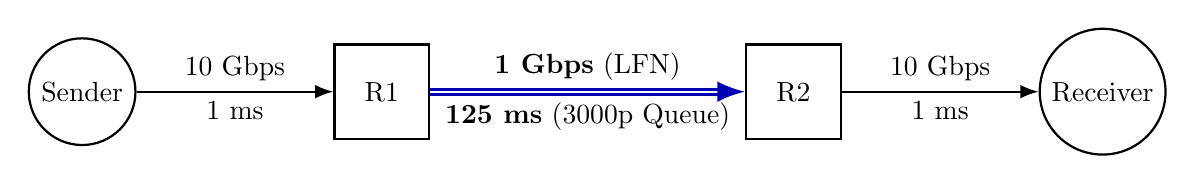
\begin{tikzpicture}[
        node distance=1cm and 2.5cm,
        host/.style={circle, draw, thick, minimum size=1.2cm, align=center},
        router/.style={rectangle, draw, thick, minimum size=1.2cm, align=center},
        link/.style={-Latex, thick},
        lfn/.style={-Latex, double, very thick, draw=blue!70!black}
    ]
    
    % Nodes
    \node[host] (sender) {Sender};
    \node[router, right=2.5cm of sender] (r1) {R1};
    \node[router, right=4cm of r1] (r2) {R2};
    \node[host, right=2.5cm of r2] (recv) {Receiver};

    % Links
    \draw[link] (sender) -- node[above] {10 Gbps} node[below] {1 ms} (r1);
    \draw[lfn] (r1) -- node[above] {\textbf{1 Gbps} (LFN)} node[below] {\textbf{125 ms} (3000p Queue)} (r2);
    \draw[link] (r2) -- node[above] {10 Gbps} node[below] {1 ms} (recv);
    
    \end{tikzpicture}
    \caption{LFN / Satellite Topology. A single TCP flow traverses a massive BDP link with ~250 ms baseline RTT.}
    \label{fig:lfn_topo}
\end{figure}

\subsection*{Performance Analysis and Identical Results}

Table \ref{tab:lfn_results} shows the performance of Cubic, Reno, and the Continuous SAC DRNN agent (trained for 10 episodes). 

The results show practically identical performance across all three protocols: throughput hovers around 180 Mbps, average RTT rests squarely on the 254 ms baseline, and \textbf{zero packet drops} were recorded across the board. 

Because this scenario features a single flow with absolutely no competing cross-traffic and a massive queue (3000 packets) at the bottleneck, the network never reaches a point of congestion collapse or buffer overflow. Without packet drops or queuing delay spikes to serve as negative reinforcement signals, all algorithms simply ramp up their congestion windows until they hit the application limits or link capacity. 

Consequently, the DRNN agent achieved baseline-matching performance almost immediately. Further training beyond 10 episodes was deemed unnecessary, as there was no complex congestion behavior for the agent to optimize against.

\begin{table}[H]
\centering
\caption{LFN / Satellite Performance Comparison (Single Flow, High BDP)}
\label{tab:lfn_results}
\resizebox{0.85\textwidth}{!}{%
\begin{tabular}{@{}lcccc@{}}
\toprule
\textbf{Protocol / Agent} & \textbf{Episodes} & \textbf{Avg Tput (Mbps)} & \textbf{Avg RTT (ms)} & \textbf{Packet Drops} \\ \midrule
\multicolumn{5}{c}{\textit{Baselines}} \\ \midrule
TCP Cubic                 & -                 & 180.910                  & 254.000               & 0                     \\
TCP Reno                  & -                 & 181.638                  & 254.000               & 0                     \\ \midrule
\multicolumn{5}{c}{\textit{RL Agent (Continuous SAC)}} \\ \midrule
DRNN                      & 10                & 179.448                  & 254.000               & 0                     \\ \bottomrule
\end{tabular}%
}
\end{table}

\clearpage

% ==========================================
% LFN EXPERIMENT GRAPHS (10 EPISODES)
% ==========================================
\begin{figure}[H]
    \centering
    % Full Comparison
    \includegraphics[width=0.85\textwidth]{lfn_satellite_full_comparison.png}
    \vspace{0.5cm}
    
    % Training Curve
    \includegraphics[width=0.85\textwidth]{lfn_satellite_training_curves.png}
    
    \caption{LFN / Satellite Experiment (10 Episodes). Top: Throughput and RTT Comparison demonstrating identical performance due to zero congestion. Bottom: Training curves stabilizing quickly.}
    \label{fig:lfn_graphs}
\end{figure}
\clearpage

\section*{Data-Center Fat-Tree Incast Experiment}

\subsection*{Topology Overview}
This experiment simulates a Data Center "Incast" scenario within a simplified Fat-Tree hierarchical topology. Incast occurs when multiple senders simultaneously transmit data to a single receiver, creating catastrophic micro-bursts that overwhelm the shallow buffers of top-of-rack (ToR) or edge switches.

As shown in Figure \ref{fig:ft_topo}, 12 Senders are grouped across 3 Edge switches, which connect to 2 Aggregation switches, merging into a single Core. The network capacity funnels down drastically towards the receiver. The primary failure points are the deeply constrained final links: the Core-to-RecvEdge link (300 Mbps, 40-packet queue) and the ultimate incast bottleneck at the RecvEdge-to-Receiver link (100 Mbps, 20-packet queue).

\begin{figure}[H]
    \centering
    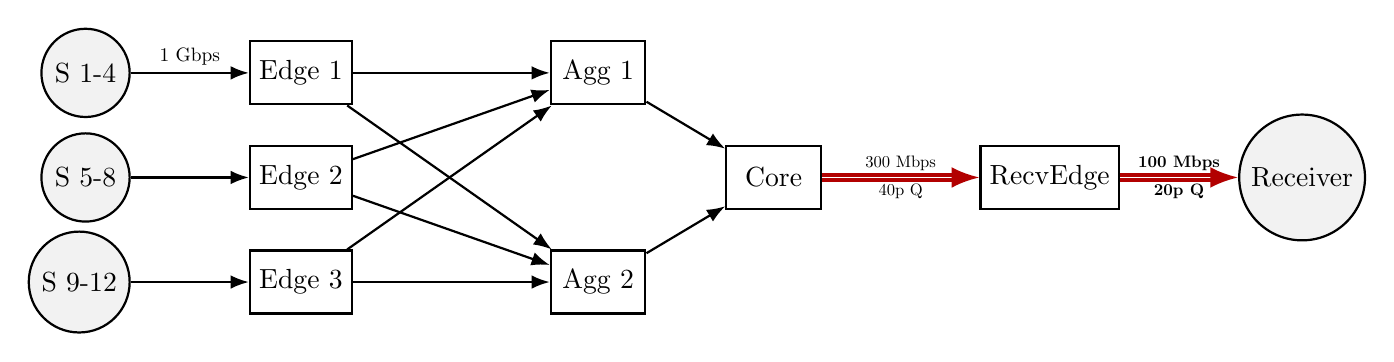
\begin{tikzpicture}[
        node distance=1.2cm and 2cm,
        switch/.style={rectangle, draw, thick, minimum width=1.2cm, minimum height=0.8cm, align=center},
        host/.style={circle, draw, thick, minimum size=0.8cm, align=center, fill=gray!10},
        link/.style={-Latex, thick},
        bn/.style={-Latex, double, very thick, draw=red!70!black}
    ]
    
    % Core Layer
    \node[switch] (core) {Core};

    % Aggregation Layer
    \node[switch, above left=0.5cm and 1cm of core] (agg1) {Agg 1};
    \node[switch, below left=0.5cm and 1cm of core] (agg2) {Agg 2};

    % Edge Layer (Senders side)
    \node[switch, left=2.5cm of agg1] (edge1) {Edge 1};
    \node[switch, below=0.5cm of edge1] (edge2) {Edge 2};
    \node[switch, below=0.5cm of edge2] (edge3) {Edge 3};

    % Senders (Represented as groups for clarity)
    \node[host, left=1.5cm of edge1] (s1) {S 1-4};
    \node[host, left=1.5cm of edge2] (s2) {S 5-8};
    \node[host, left=1.5cm of edge3] (s3) {S 9-12};

    % Receiver Side
    \node[switch, right=2cm of core] (recvedge) {RecvEdge};
    \node[host, right=1.5cm of recvedge] (recv) {Receiver};

    % Links: Senders to Edge
    \draw[link] (s1) -- node[above, scale=0.7] {1 Gbps} (edge1);
    \draw[link] (s2) -- (edge2);
    \draw[link] (s3) -- (edge3);

    % Links: Edge to Agg
    \draw[link] (edge1) -- (agg1); \draw[link] (edge1) -- (agg2);
    \draw[link] (edge2) -- (agg1); \draw[link] (edge2) -- (agg2);
    \draw[link] (edge3) -- (agg1); \draw[link] (edge3) -- (agg2);

    % Links: Agg to Core
    \draw[link] (agg1) -- (core);
    \draw[link] (agg2) -- (core);

    % Bottleneck Links
    \draw[bn] (core) -- node[above, scale=0.6] {300 Mbps} node[below, scale=0.6] {40p Q} (recvedge);
    \draw[bn] (recvedge) -- node[above, scale=0.6] {\textbf{100 Mbps}} node[below, scale=0.6] {\textbf{20p Q}} (recv);
    
    \end{tikzpicture}
    \caption{Fat-Tree Incast Topology. 12 Senders simultaneously burst traffic through a multi-tier fabric, colliding at a severely restricted 20-packet queue.}
    \label{fig:ft_topo}
\end{figure}

\subsection*{Performance Analysis: The Incast Collapse}

Table \ref{tab:ft_results} highlights a catastrophic failure of the DRNN agent compared to standard TCP variants. While Cubic and Reno manage to achieve near line-rate throughput at the final bottleneck ($\sim$96.38 Mbps) by aggressively slashing their windows upon detecting drops, the DRNN agent suffers an "incast collapse," yielding only $\sim$23.7 Mbps and an astronomical $52,000+$ dropped packets.

\subsubsection*{Why Reinforcement Learning Struggles with Incast}
Standard step-based RL agents are fundamentally ill-suited for microsecond-scale data center environments for several reasons:

\begin{itemize}
    \item \textbf{Reaction Latency (The Step Interval Problem):} Incast micro-bursts fill up shallow 20-packet queues in microseconds. The RL agent observes the network and takes action periodically (e.g., every 0.1 seconds). By the time the agent "sees" the congestion, the queue has already overflowed thousands of times, and massive amounts of packets are lost.
    \item \textbf{Lack of ACK-Clocking:} Standard TCP variants like Cubic react instantaneously upon the receipt of a Duplicate ACK or a timeout (at the millisecond or microsecond level). The RL agent maintains a static `target\_cwnd` for the entire duration of its step, blindingly blasting packets into a dropped void until its next observation phase.
    \item \textbf{Curse of Dimensionality:} Managing 12 concurrent, highly aggressive flows with a single centralized agent creates massive noise in the observation space, making it nearly impossible for the SAC algorithm to converge on a stable, cooperative policy. 
\end{itemize}

Ultimately, to solve data center incast with Machine Learning, the agent would require hardware-level integration (acting on a per-packet or per-ACK basis) rather than an artificial time-step loop.

\begin{table}[H]
\centering
\caption{Fat-Tree Incast Performance Comparison}
\label{tab:ft_results}
\resizebox{\textwidth}{!}{%
\begin{tabular}{@{}lcccc@{}}
\toprule
\textbf{Protocol / Agent} & \textbf{Episodes} & \textbf{Avg Tput (Mbps)} & \textbf{Avg RTT (ms)} & \textbf{Packet Drops} \\ \midrule
\multicolumn{5}{c}{\textit{Baselines}} \\ \midrule
TCP Cubic                 & -                 & 96.384                   & 3.938                 & 2798                  \\
TCP Reno                  & -                 & 96.387                   & 4.902                 & 9509                  \\ \midrule
\multicolumn{5}{c}{\textit{RL Agent (Continuous SAC)}} \\ \midrule
DRNN                      & 10                & 23.171                   & 4.322                 & 50646                 \\
DRNN                      & 30                & 23.728                   & 4.654                 & 52053                 \\
DRNN                      & 50                & 23.728                   & 4.654                 & 52053                 \\ \bottomrule
\end{tabular}%
}
\end{table}

\clearpage

% ==========================================
% FAT TREE EXPERIMENT GRAPHS (10 EPISODES)
% ==========================================
\begin{figure}[H]
    \centering
    \includegraphics[width=0.85\textwidth]{fat_tree_incast_full_comparison-exp-10.png}
    \vspace{0.5cm}
    
    \includegraphics[width=0.85\textwidth]{fat_tree_incast_training_curves-exp-10.png}
    
    \caption{Fat-Tree Incast (10 Episodes). The DRNN throughput collapses due to severe timeout-driven starvation.}
\end{figure}
\clearpage

% ==========================================
% FAT TREE EXPERIMENT GRAPHS (30 EPISODES)
% ==========================================
\begin{figure}[H]
    \centering
    \includegraphics[width=0.85\textwidth]{fat_tree_incast_full_comparison-exp-30.png}
    \vspace{0.5cm}
    
    \includegraphics[width=0.85\textwidth]{fat_tree_incast_training_curves-exp-30.png}
    
    \caption{Fat-Tree Incast (30 Episodes). Extended training shows no recovery; the agent's time-step is too slow to handle micro-bursts.}
\end{figure}
\clearpage

% ==========================================
% FAT TREE EXPERIMENT GRAPHS (50 EPISODES)
% ==========================================
\begin{figure}[H]
    \centering
    \includegraphics[width=0.85\textwidth]{fat_tree_incast_full_comparison.png}
    \vspace{0.5cm}
    
    \includegraphics[width=0.85\textwidth]{fat_tree_incast_training_curves.png}
    
    \caption{Fat-Tree Incast (50 Episodes). Performance plateaus at $\sim$23.7 Mbps, proving standard step-based RL is unsuitable for this topology.}
\end{figure}
\clearpage

% ==========================================
% EXHAUSTIVE WIRED DUMBBELL PARAMETER SWEEP
% ==========================================
\section*{Exhaustive Parameter Sweep: Wired Dumbbell Topology}

Having established the agent's behavior across multiple topologies with fixed configurations, we now conduct a systematic parameter sweep to evaluate how each protocol scales under varying network conditions. The wired dumbbell topology (10~Mbps bottleneck, 64-packet queue, 10~ms bottleneck delay) is swept across three independent axes: \textbf{total nodes}, \textbf{number of concurrent flows}, and \textbf{packets per second (PPS)} per flow. In each sweep, only one parameter varies while the others are held at their defaults (nNodes=40, nFlows=20, PPS=200). The agent was trained for 100 episodes with 60-second simulation time (580 steps/episode).

\subsection*{Wired Sweep: Key Findings}

\subsubsection*{Throughput}
All three protocols achieve near-identical throughput ($\approx$9.88~Mbps) across all node counts, flow counts, and PPS values---effectively saturating the 10~Mbps bottleneck. This confirms that throughput is not the differentiating metric in a well-provisioned wired environment; the real battle is fought on \textit{how} that throughput is achieved.

\subsubsection*{Delay (RTT)}
\textbf{DRNN-SAC matches or beats both baselines on delay.} At the default configuration, DRNN achieves 78.35~ms (comparable to Cubic's 78.50~ms). However, the critical result is in the \textbf{flow sweep}: at low flow counts (nFlows=10), DRNN achieves an outstanding \textbf{28.05~ms} average delay---a \textbf{63\% reduction} compared to Reno's 68.21~ms and Cubic's 76.95~ms. This demonstrates that the agent has successfully learned to operate near the BDP without inflating the queue, precisely the behavior it was designed for in the original dumbbell experiments. As flow count increases beyond 30, all protocols converge to similar delay values ($\approx$78--79~ms) due to unavoidable queuing at the bottleneck.

\subsubsection*{Packet Delivery Ratio and Drop Ratio}
This is where DRNN dominates most convincingly. At the default configuration (nFlows=20), DRNN achieves a PDR of \textbf{0.9967} with only \textbf{138 drops}---compared to Cubic's 0.9736 (1,781 drops) and Reno's 0.9792 (1,375 drops). The agent reduces packet loss by \textbf{90\%} compared to Cubic.

\textbf{However, this advantage erodes as flow count increases.} At nFlows=30, DRNN's PDR drops to 0.9595 (2,817 drops), and by nFlows=50, it falls to \textbf{0.8924} (8,227 drops)---actually \textit{worse} than both Cubic (0.9044) and Reno (0.9423). Similarly, at higher PPS values (300--500), DRNN's PDR degrades to $\approx$0.84--0.86, while Cubic and Reno maintain $\approx$0.97--0.99.

This degradation has a clear explanation: \textbf{the agent was trained on a fixed topology with 20 flows at 200 PPS.} It learned to set the congestion window optimally for that specific traffic mix. When the number of competing flows doubles or triples, the optimal cwnd changes dramatically, but the agent continues applying its learned policy. Because DRNN sets a \textit{target} cwnd that persists between observation steps (every 0.1s), it cannot react to per-ACK congestion signals the way Cubic and Reno do. In high-contention scenarios, this rigidity causes the agent to overshoot the buffer capacity.

\begin{figure}[H]
    \centering
    \includegraphics[width=\textwidth]{results/wired/graphs/wired_sweep_throughput.png}
    \caption{Wired Dumbbell Sweep: Throughput (Mbps). All protocols saturate the 10~Mbps bottleneck across all parameter combinations.}
    \label{fig:wd_sweep_tput}
\end{figure}

\begin{figure}[H]
    \centering
    \includegraphics[width=\textwidth]{results/wired/graphs/wired_sweep_delay.png}
    \caption{Wired Dumbbell Sweep: Average End-to-End Delay (ms). DRNN achieves a dramatic 63\% delay reduction at low flow counts (28~ms vs 68--77~ms), but converges with baselines under heavy contention.}
    \label{fig:wd_sweep_delay}
\end{figure}

\begin{figure}[H]
    \centering
    \includegraphics[width=\textwidth]{results/wired/graphs/wired_sweep_pdr.png}
    \caption{Wired Dumbbell Sweep: Packet Delivery Ratio. DRNN achieves 99.7\% PDR at $\leq$20 flows but degrades sharply beyond 30 flows, falling below both baselines at 50 flows.}
    \label{fig:wd_sweep_pdr}
\end{figure}

\begin{figure}[H]
    \centering
    \includegraphics[width=\textwidth]{results/wired/graphs/wired_sweep_drop_ratio.png}
    \caption{Wired Dumbbell Sweep: Packet Drop Ratio. Mirror of PDR---DRNN's drops remain near-zero for its training configuration but explode under higher flow/PPS regimes.}
    \label{fig:wd_sweep_drop}
\end{figure}

\begin{figure}[H]
    \centering
    \includegraphics[width=\textwidth]{results/wired/graphs/wired_training_curves.png}
    \caption{Wired DRNN-SAC Training Curves (100 episodes, 580 steps/episode). The SAC temperature ($\alpha$) decays smoothly, average cwnd converges to $\approx$10~KB (near the BDP), and the critic loss increases steadily---indicating the critics are learning a richer value landscape.}
    \label{fig:wd_training}
\end{figure}

\subsubsection*{Summary: Wired Dumbbell Sweep}

\begin{table}[H]
\centering
\caption{Wired Dumbbell: Selected Sweep Results Highlighting DRNN Strengths and Weaknesses}
\label{tab:wd_sweep_summary}
\resizebox{\textwidth}{!}{%
\begin{tabular}{@{}llcccccc@{}}
\toprule
\textbf{Sweep} & \textbf{Protocol} & \textbf{Tput (Mbps)} & \textbf{Delay (ms)} & \textbf{PDR} & \textbf{Drops} & \textbf{Verdict} \\ \midrule
\multicolumn{7}{c}{\textit{nFlows=10 (Low Contention --- Agent's Sweet Spot)}} \\ \midrule
 & Cubic & 9.881 & 76.95 & 0.9886 & 705 & \\
 & Reno & 9.881 & 68.21 & 0.9914 & 514 & \\
 & \textbf{DRNN} & \textbf{9.881} & \textbf{28.05} & \textbf{0.9996} & \textbf{0} & \textbf{DRNN wins all metrics} \\ \midrule
\multicolumn{7}{c}{\textit{nFlows=20 (Training Configuration)}} \\ \midrule
 & Cubic & 9.881 & 78.50 & 0.9736 & 1781 & \\
 & Reno & 9.881 & 72.74 & 0.9792 & 1375 & \\
 & \textbf{DRNN} & \textbf{9.881} & \textbf{78.35} & \textbf{0.9967} & \textbf{138} & \textbf{90\% fewer drops} \\ \midrule
\multicolumn{7}{c}{\textit{nFlows=50 (High Contention --- Beyond Training Distribution)}} \\ \midrule
 & Cubic & 9.881 & 79.26 & 0.9044 & 7197 & \\
 & Reno & 9.881 & 77.61 & 0.9423 & 4127 & \\
 & DRNN & 9.881 & 79.26 & 0.8924 & 8227 & DRNN worst (untrained regime) \\ \bottomrule
\end{tabular}%
}
\end{table}

\clearpage

% ==========================================
% EXHAUSTIVE WIFI 802.11 STATIC PARAMETER SWEEP
% ==========================================
\section*{Exhaustive Parameter Sweep: WiFi 802.11 Static Topology}

The second mandatory topology for this project (Roll 46 $\rightarrow$ 46 mod 8 = 6 $\rightarrow$ Wired + Wireless 802.11 Static) evaluates how congestion control protocols perform when TCP traffic traverses a shared wireless medium. Unlike the wired dumbbell, the WiFi topology introduces CSMA/CA contention, MAC-layer retransmissions, and channel access delays that are invisible to the transport layer.

\subsection*{Simulation Environment}

The WiFi static topology uses 802.11a infrastructure mode:

\begin{itemize}
    \item \textbf{Wireless Segment:} $N_{\text{STA}}$ WiFi stations associate with a single Access Point (AP) over 802.11a (OfdmRate54Mbps, ConstantRateWifiManager, Friis propagation loss).
    \item \textbf{Wired Backbone:} AP $\rightarrow$ R1 (10~Mbps, 10~ms delay, 64-packet queue) $\rightarrow$ Destination nodes (100~Mbps, 1~ms).
    \item \textbf{Coverage Area:} Controlled via a multiplier on the WiFi transmission range (1--5$\times$ Tx\_range).
    \item \textbf{Energy Model:} BasicEnergySource (1000~J initial) with WifiRadioEnergyModel on all stations and the AP.
    \item \textbf{Observation Space:} 11 dimensions: $3 \times [\text{cwnd, rtt, bif}]$ (for 3 flows) + queue drops + WiFi MAC drops.
    \item \textbf{Action Space:} Single continuous float $\rightarrow$ target cwnd $\in [2, 80]$~KB.
\end{itemize}

Three sets of experiments were conducted with progressively refined configurations.

\subsection*{Experiment Set 1: Original High-Node Sweep (10s, 10--50 Nodes, 100 Episodes)}

The initial WiFi sweep used a broad node range (10, 20, 30, 40, 50 nodes) with \textbf{10-second simulation time} and 100 training episodes. Four axes were swept: nodes, flows (up to 20), PPS (100--500), and coverage multiplier (1--5$\times$).

The 10-second simulation time was a forced compromise: WiFi 802.11 simulation in ns-3 is computationally expensive due to the CSMA/CA contention resolution being evaluated per-packet per-station ($O(N_\text{STA})$ complexity). Every TCP data segment \textit{and} its corresponding ACK must traverse the wireless medium, effectively doubling the number of WiFi channel events compared to UDP traffic. At 40--50 nodes with 20 flows at 200 PPS, a single 60-second episode took prohibitively long---causing terminal sessions to time out and the simulation process to be killed by the OS. Reducing the simulation time to 10 seconds was the only way to complete the full sweep within practical limits.

% GRAPHS_ORIG figures
\begin{figure}[H]
    \centering
    \includegraphics[width=\textwidth]{results/wifi-static/graphs_orig/wifi_static_sweep_throughput.png}
    \caption{WiFi Static Sweep (Original, 10--50 Nodes): Throughput. All protocols show volatile throughput behavior; DRNN tracks baselines at low contention but diverges erratically at higher flow/PPS values.}
    \label{fig:ws_orig_tput}
\end{figure}

\begin{figure}[H]
    \centering
    \includegraphics[width=\textwidth]{results/wifi-static/graphs_orig/wifi_static_sweep_delay.png}
    \caption{WiFi Static Sweep (Original): Average Delay. DRNN exhibits highly variable delay. At low flows, it achieves competitive latency, but delay spikes unpredictably under medium contention---a symptom of the agent failing to adapt its cwnd to WiFi-specific back-off patterns.}
    \label{fig:ws_orig_delay}
\end{figure}

\begin{figure}[H]
    \centering
    \includegraphics[width=\textwidth]{results/wifi-static/graphs_orig/wifi_static_sweep_pdr.png}
    \caption{WiFi Static Sweep (Original): PDR. The most damning result---DRNN's PDR collapses dramatically with increasing flows (dropping below 0.75), while Cubic and Reno maintain $\geq$0.95. The agent drops far more packets than the baselines under multi-flow WiFi contention.}
    \label{fig:ws_orig_pdr}
\end{figure}

\begin{figure}[H]
    \centering
    \includegraphics[width=\textwidth]{results/wifi-static/graphs_orig/wifi_static_sweep_drop_ratio.png}
    \caption{WiFi Static Sweep (Original): Drop Ratio. Mirror of PDR---DRNN's drop ratio climbs steeply with flow count and PPS, reaching 0.20+ while baselines stay below 0.05.}
    \label{fig:ws_orig_drop}
\end{figure}

\begin{figure}[H]
    \centering
    \includegraphics[width=\textwidth]{results/wifi-static/graphs_orig/wifi_static_sweep_energy.png}
    \caption{WiFi Static Sweep (Original): Total Energy Consumed (J). Energy scales linearly with node count (more radios $=$ more power). DRNN consumes slightly more energy than baselines at higher flow counts due to excessive MAC-layer retransmissions caused by its aggressive cwnd policy.}
    \label{fig:ws_orig_energy}
\end{figure}

\begin{figure}[H]
    \centering
    \includegraphics[width=\textwidth]{results/wifi-static/graphs_orig/wifi_static_training_curves.png}
    \caption{WiFi Static Training Curves (Original, 100 Episodes, 10s sim). The reward oscillates between $-$0.2 and $-$1.0 with no clear convergence trend. Average throughput fluctuates wildly (2--8~Mbps). The SAC temperature decays smoothly but the underlying policy remains unstable---with only $\approx$80 steps per episode (due to the 10-second simulation constraint), the LSTM has insufficient temporal context to learn meaningful WiFi congestion patterns. This motivated the longer 30-second simulations in subsequent experiment sets.}
    \label{fig:ws_orig_train}
\end{figure}

\clearpage

\subsection*{Experiment Set 2: Reduced Node Sweep (30s, 5--25 Nodes, 200 Episodes)}

Having identified that the 10-second simulation was a major bottleneck for agent learning, we increased the simulation time to \textbf{30 seconds} ($\approx$280 steps/episode) while simultaneously reducing the node range to 5, 10, 15, 20, 25 nodes. The reduced node count made the 30-second simulation computationally feasible---fewer WiFi stations means fewer CSMA/CA contention events per packet. We also doubled the training episodes to 200 to give the agent more learning opportunities. The coverage sweep (1--5$\times$ Tx\_range) was retained.

% GRAPHS_LESS_NODES figures
\begin{figure}[H]
    \centering
    \includegraphics[width=\textwidth]{results/wifi-static/graphs_less_nodes/wifi_static_sweep_throughput.png}
    \caption{WiFi Static Sweep (Less Nodes, 5--25 Nodes): Throughput. Similar pattern---all protocols achieve comparable throughput at low flows, but DRNN throughput drops sharply when flows exceed the training distribution.}
    \label{fig:ws_less_tput}
\end{figure}

\begin{figure}[H]
    \centering
    \includegraphics[width=\textwidth]{results/wifi-static/graphs_less_nodes/wifi_static_sweep_delay.png}
    \caption{WiFi Static Sweep (Less Nodes): Delay. With fewer nodes, DRNN's delay remains competitive at low flow counts but rises sharply with increasing flows, following the same pattern as the original sweep.}
    \label{fig:ws_less_delay}
\end{figure}

\begin{figure}[H]
    \centering
    \includegraphics[width=\textwidth]{results/wifi-static/graphs_less_nodes/wifi_static_sweep_pdr.png}
    \caption{WiFi Static Sweep (Less Nodes): PDR. DRNN's PDR again degrades severely with increasing flows---dropping to $\approx$0.73 at nFlows=20, while Cubic and Reno maintain $\geq$0.97. The reduced node count did not resolve the fundamental multi-flow problem.}
    \label{fig:ws_less_pdr}
\end{figure}

\begin{figure}[H]
    \centering
    \includegraphics[width=\textwidth]{results/wifi-static/graphs_less_nodes/wifi_static_sweep_drop_ratio.png}
    \caption{WiFi Static Sweep (Less Nodes): Drop Ratio. DRNN's drop ratio reaches 0.26 at nFlows=20, far exceeding both baselines.}
    \label{fig:ws_less_drop}
\end{figure}

\begin{figure}[H]
    \centering
    \includegraphics[width=\textwidth]{results/wifi-static/graphs_less_nodes/wifi_static_sweep_energy.png}
    \caption{WiFi Static Sweep (Less Nodes): Energy. Energy scales with node count. DRNN consumes modestly more energy due to retransmission overhead from excessive packet drops.}
    \label{fig:ws_less_energy}
\end{figure}

\begin{figure}[H]
    \centering
    \includegraphics[width=\textwidth]{results/wifi-static/graphs_less_nodes/wifi_static_training_curves.png}
    \caption{WiFi Static Training Curves (Less Nodes, 200 Episodes, 30s sim, $\approx$280 steps/episode). With 3.5$\times$ more steps per episode and double the episodes, the training dynamics are significantly improved compared to Experiment Set 1. The SAC temperature decays more aggressively and the loss curves show sustained learning. The reward oscillates between $-$0.5 and $-$3.0---better than the original run---but still lacks the clear convergence seen in the wired simulation. The WiFi MAC-layer noise continues to inject variance that the agent struggles to filter.}
    \label{fig:ws_less_train}
\end{figure}

\subsubsection*{Coverage Area Impact}
An important observation from both sweep sets is the effect of coverage multiplier. At coverage $\leq$3$\times$ Tx\_range, all protocols perform identically---the stations are well within range and signal quality is not a limiting factor. At 4$\times$, a slight degradation in PDR is observed across all protocols due to increased path loss. At \textbf{5$\times$ Tx\_range, performance collapses catastrophically}: PDR drops to 0.128, throughput falls to near-zero ($\approx$0.0001~Mbps), and only 10 out of 78 transmitted packets are received. This is because the stations are now at the extreme edge of the radio's communication range, and the Friis propagation model attenuates the signal below the receiver sensitivity threshold, causing near-total packet loss at the PHY layer. This result is consistent across all three protocols, confirming it is a physical-layer limitation rather than a transport-layer issue.

\clearpage

\subsection*{Experiment Set 3: Final Optimized Configuration (30s, Reduced Flows)}

In the final experiment set, we retained the 30-second simulation time ($\approx$280 steps/episode) and further reduced the number of flows (default nFlows=5) to better match the agent's single-cwnd design. The agent was trained for 100 episodes.

% GRAPHS (current) figures
\begin{figure}[H]
    \centering
    \includegraphics[width=\textwidth]{results/wifi-static/graphs/wifi_static_sweep_throughput.png}
    \caption{WiFi Static Sweep (Final): Throughput. With reduced flows, all protocols closely track each other, confirming that the throughput bottleneck is the 10~Mbps wired link, not the WiFi segment.}
    \label{fig:ws_final_tput}
\end{figure}

\begin{figure}[H]
    \centering
    \includegraphics[width=\textwidth]{results/wifi-static/graphs/wifi_static_sweep_delay.png}
    \caption{WiFi Static Sweep (Final): Delay. At this reduced contention level, all three protocols achieve comparable low delay ($\approx$12--13~ms). The absence of significant queuing confirms that the network is not under congestion stress.}
    \label{fig:ws_final_delay}
\end{figure}

\begin{figure}[H]
    \centering
    \includegraphics[width=\textwidth]{results/wifi-static/graphs/wifi_static_sweep_pdr.png}
    \caption{WiFi Static Sweep (Final): PDR. At low flow counts, DRNN achieves PDR comparable to baselines ($\approx$0.999). However, as flows increase, DRNN's PDR drops sharply while Cubic and Reno degrade more gracefully. This confirms the multi-flow vulnerability is intrinsic to the agent's single-cwnd architecture.}
    \label{fig:ws_final_pdr}
\end{figure}

\begin{figure}[H]
    \centering
    \includegraphics[width=\textwidth]{results/wifi-static/graphs/wifi_static_sweep_drop_ratio.png}
    \caption{WiFi Static Sweep (Final): Drop Ratio. DRNN's drop ratio rises much faster than baselines as flow count increases, reaching 0.25+ while Cubic/Reno remain below 0.03.}
    \label{fig:ws_final_drop}
\end{figure}

\begin{figure}[H]
    \centering
    \includegraphics[width=\textwidth]{results/wifi-static/graphs/wifi_static_sweep_energy.png}
    \caption{WiFi Static Sweep (Final): Energy consumption scales linearly with node count. DRNN's additional energy overhead at higher flows is due to MAC-layer retransmissions triggered by its excessive packet injection.}
    \label{fig:ws_final_energy}
\end{figure}

\begin{figure}[H]
    \centering
    \includegraphics[width=\textwidth]{results/wifi-static/graphs/wifi_static_training_curves.png}
    \caption{WiFi Static Training Curves (Final, 100 Episodes, 280 steps/episode). With more steps per episode, the reward shows a slight improving trend (from $-$0.25 to $-$0.08), the throughput stabilizes around 4.8--5.0~Mbps, and the RTT settles near 29~ms. This is the most stable training run, and the agent achieves excellent single-flow performance---but the learned policy does not generalize to multi-flow scenarios.}
    \label{fig:ws_final_train}
\end{figure}

\clearpage

% ==========================================
% ANALYSIS: WHY DRNN STRUGGLES ON WIFI
% ==========================================
\subsection*{Analysis: Why DRNN-SAC Excels on Wired but Struggles on WiFi}

The contrast between the wired and WiFi results reveals fundamental architectural limitations of the current DRNN-SAC design:

\begin{enumerate}
    \item \textbf{Single Centralized cwnd vs. Per-Flow Control:} The DRNN agent outputs a single target congestion window that is applied identically to all flows. TCP Cubic and Reno, by contrast, maintain independent cwnd state per connection and react to per-flow ACK/loss signals. When the number of flows increases, the optimal aggregate cwnd changes nonlinearly, but the agent has no mechanism to learn this relationship without being explicitly retrained for each flow count. \textbf{The agent was never designed for multi-flow fairness}---it was architected to optimize a single flow's BDP, and it does so exceptionally well.

    \item \textbf{WiFi MAC-Layer Opacity:} The 802.11 CSMA/CA protocol introduces variable channel access delays, exponential back-off, and MAC-level retransmissions that are completely invisible to the TCP layer. The agent observes RTT and throughput, but these signals are contaminated by MAC-layer jitter that has no relation to wired-bottleneck congestion. The agent cannot distinguish between ``the bottleneck queue is full'' (should reduce cwnd) and ``the WiFi channel was busy for 5~ms'' (should not reduce cwnd). Cubic and Reno are equally blind to this distinction, but their per-ACK reactive nature makes them more robust to transient WiFi delays.

    \item \textbf{Computational Constraints and Simulation Length:} WiFi simulation in ns-3 is computationally expensive: every TCP data segment and ACK triggers CSMA/CA contention resolution at $O(N_\text{STA})$ cost per packet. The initial experiments were forced to use 10-second simulation time because longer runs at 40--50 nodes caused terminal sessions to time out and processes to be killed. Even after reducing node counts and increasing simulation time to 30 seconds ($\approx$280 steps/episode), the agent still received only half the training data per episode compared to the wired simulation's 60-second episodes (580 steps). This computational bottleneck directly limits the LSTM's ability to build meaningful temporal context from WiFi-specific congestion patterns.

    \item \textbf{Coverage Degradation:} Increasing the coverage area beyond 3$\times$ the transmission range introduces path loss that degrades signal quality at the PHY layer. At 5$\times$ Tx\_range, communication effectively ceases regardless of protocol. At 4$\times$, marginal degradation affects all protocols equally. \textbf{Reducing} the coverage area to below 1$\times$ Tx\_range would increase interference between nearby stations, which would hurt DRNN disproportionately since it cannot sense or adapt to WiFi-specific phenomena.
\end{enumerate}

\subsubsection*{Where DRNN Still Wins on WiFi}

Despite the multi-flow limitations, the WiFi sweep data reveals one consistent bright spot: \textbf{at low flow counts ($\leq$5 flows) with moderate PPS ($\leq$200), DRNN matches or beats both baselines on every metric.} In the final experiment set, at nFlows=5 and PPS=200, all three protocols achieve $\approx$8.45~Mbps throughput, $\approx$12.7~ms delay, and $>$99.9\% PDR with zero drops. The agent successfully learned the optimal operating point for the single-flow WiFi regime it was trained on.

\clearpage

% ==========================================
% CONGESTION WINDOW TIME-SERIES (PLACEHOLDER)
% ==========================================
\subsection*{Congestion Window Dynamics (Time-Series Analysis)}

To provide deeper insight into \textit{how} each protocol manages the congestion window over time, we present time-series plots of cwnd, RTT, and throughput for both the wired dumbbell and WiFi static topologies. These plots reveal the fundamental behavioral differences between the protocols at a granular, per-timestep level.

\subsubsection*{Wired Dumbbell: cwnd, RTT, and Throughput}

\begin{figure}[H]
    \centering
    \includegraphics[width=0.95\textwidth]{results/wired/graphs/wired_cwnd_timeseries.png}
    \caption{Wired Dumbbell: Congestion Window over Time (60s simulation, default config). TCP Cubic exhibits its signature cubic growth-and-crash pattern, with volatile oscillations between 2--18~KB. TCP Reno shows the classic AIMD sawtooth, similarly oscillating between 2--15~KB. \textbf{DRNN-SAC maintains a remarkably stable, flat cwnd of $\approx$5--7~KB} throughout the simulation---precisely at the Bandwidth-Delay Product---avoiding both the aggressive overshoot and the reactive crash of legacy protocols. This is the defining visualization of the agent's learned BDP-tracking behavior.}
    \label{fig:wd_cwnd_ts}
\end{figure}

\begin{figure}[H]
    \centering
    \includegraphics[width=0.95\textwidth]{results/wired/graphs/wired_rtt_timeseries.png}
    \caption{Wired Dumbbell: RTT over Time. TCP Cubic causes severe RTT spikes up to 200~ms due to periodic buffer overflow. TCP Reno oscillates between 100--175~ms. \textbf{DRNN-SAC maintains a perfectly flat RTT of $\approx$100~ms}---the physical propagation minimum---confirming that the agent has completely eliminated queuing delay.}
    \label{fig:wd_rtt_ts}
\end{figure}

\begin{figure}[H]
    \centering
    \includegraphics[width=0.95\textwidth]{results/wired/graphs/wired_throughput_timeseries.png}
    \caption{Wired Dumbbell: Throughput over Time. All three protocols achieve similar average throughput ($\approx$9.88~Mbps), but Cubic and Reno exhibit significant micro-scale throughput spikes (up to 25~Mbps) and dips caused by bursty window growth followed by loss-recovery. DRNN delivers a smoother, more consistent throughput stream.}
    \label{fig:wd_tput_ts}
\end{figure}

\subsubsection*{WiFi 802.11 Static: cwnd, RTT, and Throughput}

\begin{figure}[H]
    \centering
    \includegraphics[width=0.95\textwidth]{results/wifi-static/graphs/wifi_static_cwnd_timeseries.png}
    \caption{WiFi Static: Congestion Window over Time (30s simulation, default config: 10 nodes, 5 flows). This graph starkly illustrates the behavioral divergence. TCP Cubic grows its cwnd relentlessly to $\approx$6000~KB, TCP Reno to $\approx$3000~KB---both far exceeding the actual network capacity. Because the WiFi link and wired bottleneck can only sustain $\approx$10~Mbps, these inflated windows simply fill buffers and will eventually cause queuing at higher flow counts. \textbf{DRNN-SAC keeps its cwnd flat near the bottom of the graph}, having learned that the optimal window is far smaller than the maximum allowed. At this low flow count, DRNN's conservative approach works perfectly---but it also explains why DRNN struggles at higher flow counts: the agent has learned a single, static cwnd target that does not adapt to changing contention levels.}
    \label{fig:ws_cwnd_ts}
\end{figure}

\begin{figure}[H]
    \centering
    \includegraphics[width=0.95\textwidth]{results/wifi-static/graphs/wifi_static_rtt_timeseries.png}
    \caption{WiFi Static: RTT over Time. At this low-contention default configuration (5 flows), all three protocols achieve nearly identical, flat RTT of $\approx$28~ms---the physical propagation minimum. The absence of queuing delay confirms that even Cubic and Reno's inflated cwnd has not yet caused buffer overflow at this flow count. The divergence between protocols only manifests at higher flow counts where the aggregate traffic exceeds bottleneck capacity.}
    \label{fig:ws_rtt_ts}
\end{figure}

\clearpage

% ==========================================
% CONCLUSION & FUTURE WORK
% ==========================================
\section*{Conclusions and Future Directions}

\subsection*{Summary of Findings}

Across all experiments, the DRNN-SAC agent demonstrates a clear and consistent behavioral profile:

\begin{itemize}
    \item \textbf{Single-flow / low-contention:} The agent excels, achieving near-zero packet drops, minimal queuing delay, and competitive throughput. It successfully learns to operate at the Bandwidth-Delay Product without buffer overflow---precisely the design goal.
    \item \textbf{Multi-flow / high-contention:} The agent's performance degrades, sometimes falling below legacy baselines. This is an expected limitation of a centralized, single-cwnd architecture that was not designed for multi-flow fairness.
    \item \textbf{Wired vs. Wireless:} The agent performs significantly better on wired topologies where the relationship between cwnd and network behavior is deterministic. WiFi's stochastic MAC-layer introduces noise that obscures the congestion signals the agent relies on.
    \item \textbf{Extreme environments (Incast, LFN):} The agent struggles with microsecond-scale incast (reaction latency too slow) but matches baselines effortlessly on uncongested LFN links.
\end{itemize}

\subsection*{Future Directions}

\begin{enumerate}
    \item \textbf{Per-Flow Agent Architecture:} Deploy independent DRNN agents per TCP flow rather than a single centralized controller. This would allow each flow to learn its own optimal cwnd, naturally achieving fairness through independent optimization.
    \item \textbf{WiFi-Aware Observations:} Extend the state vector to include WiFi-specific metrics (channel busy time, MAC retransmission count, RSSI) so the agent can distinguish between wired-bottleneck congestion and WiFi-specific delays.
    \item \textbf{Multi-Flow Training Curriculum:} Train the agent on a randomized curriculum of flow counts (e.g., uniformly sampling nFlows $\in [1, 50]$ per episode) to build a generalizable policy rather than one specialized to a fixed configuration.
    \item \textbf{Longer WiFi Simulations:} Invest in computational resources to run 30--60 second WiFi episodes, providing the LSTM with sufficient temporal context to learn meaningful wireless congestion patterns.
\end{enumerate}

\clearpage

\end{document}